\section{K Shortest Path}

\begin{frame}[plain]{}
    \sectionpage
\end{frame}

\begin{frame}[allowframebreaks]{Introduction}
    Let $G=(V,E)$ be a directed weighed graph, where $V$ is the set of nodes and $E \subseteq V \times V$ be the set of arcs. 
    
    \begin{block}{Problem}
    The K shortest path problem consists in enumerating, in order of increasing length, the K paths from the starting node $s$ to a terminal node $t$ with minimum total length.
    \end{block}
    
    We can assume that the graph is acyclic and that there are no negative weights.
    
    \framebreak
    Here, we report a list of relevant definition, useful later on:
    \begin{itemize}
        \item Given an arc $e=(u,v) \in E$, we can define $tail(e)=u$ and $head(e)=v$.
        \item A path from $u$ to $v$ is a sequence of arcs $p=p_1\cdot p_2 \dots p_{|p|}$ such that $tail(p_1)=u$ and $head(p_{|p|})=v$.
        \item Let $T$ be the single-destination shortest path tree containing the shortest path from every node $v \in V$ to $t$.
        \item Let $out(v)$ be the set of arcs with tail $v$ that are not in the shortest path from $v$ to $t$
        \item Let $next_T(v)$ be the node $w$ following $v$ in $T$ (so, the shortest path from $v$ to $t$ is made by $(v,w)$ followed by the shortest path from $w$ to $t$).
        \item $\forall e=(u,v) \in E$ let $\delta(u,v) = \ell(u,v) + d(v,t) - d(u,t)$ where $\ell(u,v)$ is the weight associated to the edge $e$ while $d(j,t)$ is the length of the shortest path from node $j$ to $t$. $\delta(u,v)$ is defined as the sidetrack weight, that is the additional cost that we have to pay if we want to reach $t$ from $u$ by following arc $e$ instead of the shortest path $u-t$
        \item If $(u,v) \in E$ and $\delta(u,v)>0$, then $(u,v)$ is called a sidetrack edge
    \end{itemize}
    
\end{frame}

\begin{frame}[allowframebreaks]{Eppstein algorithm: basic idea}
    \begin{enumerate}
        \item We compute $T$ and $\forall e=(u,v) \in E$ $\delta(u,v)$. This can be done through the Dijkstra algorithm (implemented in the Shortest\_path\_finder class)
        \item $\forall v \in V$ we compute $H_{out}(v)$, a modified binary heap in which the elements are the edges in the outer star of $v$, ordered by sidetrack weight. $H_{out}(v)$ is constructed in such a way that the first node, called $outroot(v)$ has a single child.
        
        \begin{figure}
            \centering
            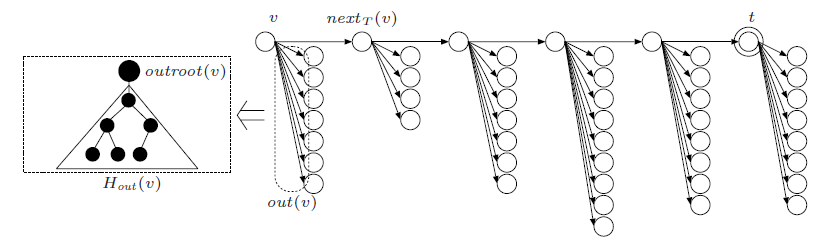
\includegraphics[width=0.7\linewidth]{Img/k_finder/h_out.PNG}
            \caption{$H_{out}(v)$ construction}
        \end{figure}
        
        \framebreak
        
        \item If $v=t$, $H_G(v)$ is a binary heap whose only element is $H_{out}(v)$; else, $H_G(v)$ is built by inserting $H_{out}(v)$ into $H_G(next_T(v))$ with weight $\ell(sidetrack(v))$. The root of $H_G(v)$ is denoted as $h(v)$
        
        \begin{figure}
            \centering
            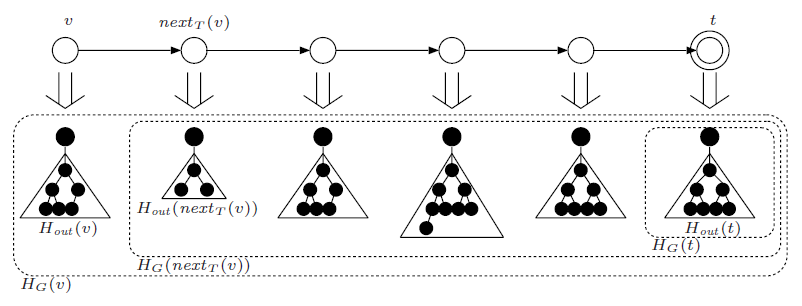
\includegraphics[width=0.7\linewidth]{Img/k_finder/h_g.PNG}
            \caption{$H_{G}(v)$ construction}
        \end{figure}
        
        \framebreak
        
        \begin{figure}
            \centering
            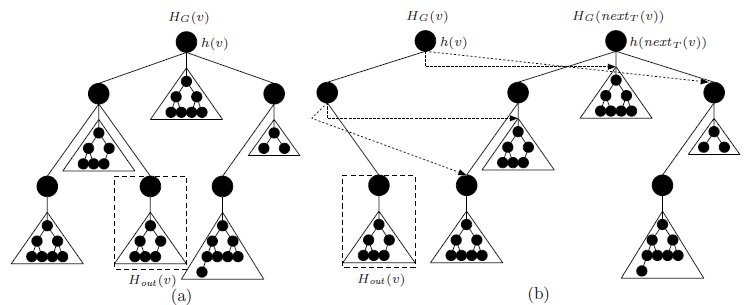
\includegraphics[width=0.7\linewidth]{Img/k_finder/h_out_h_g.PNG}
            \caption{(a) $H_G(v)$; (b) $H_G(v)$ with references to the different $H_{out}(v)$}
        \end{figure}
        
        \framebreak
        
        \item The set of all $H_G(v)$ for all $v \in V$ forms a directed acyclic graph $D(G)$. Each node in $D(G)$ corresponds to an edge in $G$ and each arc in $G$ is represented by at least one node in $D(G)$. $\forall (e,f)$ in which $e$ is the parent of $f$ in any heap $H_G(v)$, there is an edge in $D(G)$.
        \item We have then to execute the following algorithm to find the K shortest paths:
        \begin{enumerate}
            \item Initialize a priority queue $Q$ to ${h(s)}$
            \item For $k = 2$ to K:
            \begin{enumerate}
                \item If $Q$ is empty, stop (no more paths exist); else, extract $S^k$, the element in $Q$ with the lowest score. Let $e$ be the last sidetrack of $S^k$.
                \item Insert $S^k \cdot f$ in $Q$ with score $L(S^k) + \delta(f)$, where $f$ is the sidetrack $h(head(e))$ and $L(S^k)$ is the sum of all the sidetrack weights of all the sidetrack edges in $S^k$
                \item For each sidetrack $f$ such that $(e,f)$ is an arc in the graph $D(G)$, insert $prefix(S^k) \cdot f$ in $Q$ with score $L(S^k)-\delta(e)+\delta(f)$, where $prefix(S^k)$ is the sequence $S^k$ except its last sidetrack
            \end{enumerate}
        \end{enumerate}
        \item Finally, by using the equivalence between a collection of sidetrack edges and a path, we can reconstruct the K shortest paths.
    \end{enumerate}
\end{frame}

\begin{frame}{Lazy Eppstein algorithm: basic idea}
    We can notice that during step 5 we only need $h(s)$ (and thus $H_G(s)$ and the related $H_{out}(v)$ for every $v$ in the shortest path $s-t$) and $H_G(head(e))$. Thus, we could construct an alternative algorithm that generates the needed $H_{out}(v)$, $H_G(v)$ and, thus, $D(G)$ during the 5th step itself. This new algorithm is called Lazy Eppstein algorithm.

    
    In this way, the worst case complexity of the method doesn't change, and, unless the number of requested paths is particularly high, the overall execution time of the Lazy Eppstein algorithm is smaller than the classic version.
\end{frame}
